\documentclass{ximera}

\author{Anna Davis} \title{MTH 140 Homework 10} 

\begin{document}

\begin{abstract}

\end{abstract}
\maketitle
% \textit{Certificate due: 12/4/2020 at 11:59 p.m.}
\begin{problem}\label{prob:140hom10prob1}

Twenty nine subjects aged 17 through 69 had their systolic blood pressure checked.  The results are recorded in \href{https://docs.google.com/spreadsheets/d/1v_i5UPj_IH2-d8QphkCZJiPbK0oV1fd0NAXmLnT8hnE/edit?usp=sharing}{BLOOD PRESSURE DATA}.  (Copy this data to a spreadsheet of your choice.)
\begin{enumerate}
    \item Find the equation for the line of best fit.
    $$y=\answer[tolerance=0.001]{0.949}x+\answer[tolerance=0.1]{97.1}$$
    \item Find the coefficient of determination. (Round to three decimal places.)
    $$r^2=\answer[tolerance=0.001]{0.712}$$
    Interpret $r^2$.
    \begin{multipleChoice} 
    \choice{The value of $r^2$ is not close to 1, so the correlation between age and systolic blood pressure is weak.} 
    \choice{Approximately $70\%$ of study participants had higher-than-normal blood pressure.}
    \choice{Blood pressure accounts for approximately $49\%$ of variability in age.}
\choice[correct]{Age accounts for approximately $70\%$ of variability in systolic blood pressure.}  
\end{multipleChoice} 
    \item Find the correlation coefficient.  (Round to two decimal places.)
    $$r=\answer[tolerance=0.01]{0.84}$$
    Classify the correlation between age and systolic blood pressure.
    
    \begin{multipleChoice} 
\choice[correct]{Strong, positive.}  
\choice{Strong, negative.} 
\choice{Weak, positive.} 
\choice{Weak, negative.}  
\end{multipleChoice}  
\item Use your linear regression equation to estimate systolic blood pressure for a 46 year old individual.  

Systolic blood pressure: $\answer[tolerance=0.1]{140.8}$
\item Select the most accurate statement regarding making predictions about systolic blood pressure of a 75 year old individual.
\begin{multipleChoice} 
\choice{We cannot make predictions about blood pressure because of significant variations among individuals.}
\choice{We can predict this individual's blood pressure by plugging 75 into the linear regression equation.}  
\choice{We cannot accurately predict the blood pressure of a 75 year old because none of the 29 subjects were 75 years old.} 
\choice[correct]{Plugging 75 into the linear regression equation will not produce reliable results because 75 is outside of the age range of study participants.} 
\end{multipleChoice}  
\end{enumerate}
\end{problem}

\begin{problem}\label{prob:140hom10prob2}
Use the screenshot below to answer the question.  

\begin{center}
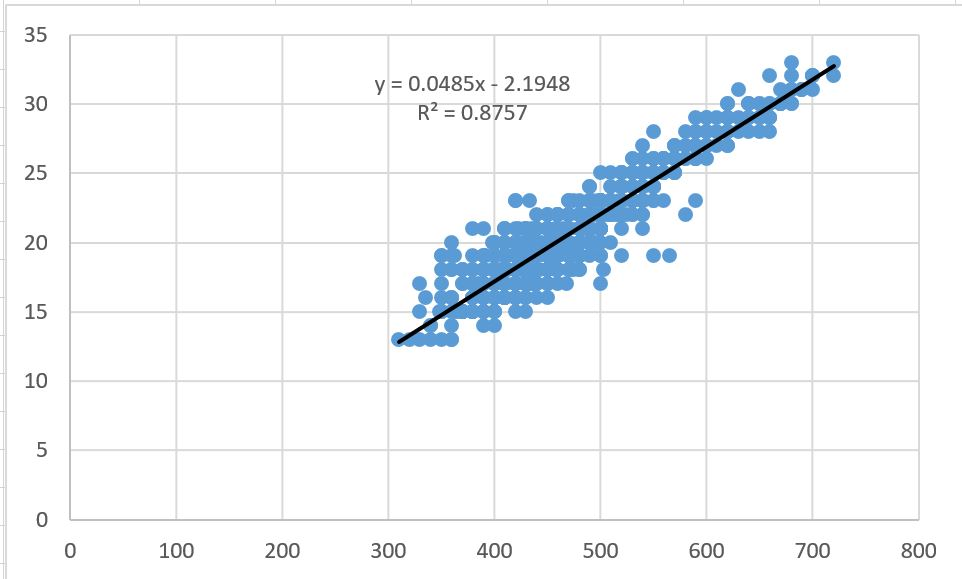
\includegraphics[height=2in]{140H10pic1.jpg}
\end{center}

Compute the correlation coefficient $r$.
 $$r=\answer[tolerance=0.01]{0.9378}$$
\end{problem}
\end{document} 


